\documentclass{beamer}
\usepackage{tcolorbox}
\usepackage{caption}
%\beamerdefaultoverlayspecification{<+->}
\newcommand{\data}{\mathcal{D}}
\usepackage{amsmath}
\usepackage{pdfpages}

\DeclareMathOperator*{\argmin}{arg\,min}

\newcommand\Item[1][]{%
	\ifx\relax#1\relax  \item \else \item[#1] \fi
	\abovedisplayskip=0pt\abovedisplayshortskip=0pt~\vspace*{-\baselineskip}}


\usetheme{metropolis}           % Use metropolis theme


\title{Coordinate Descent}
\date{\today}
\author{Nipun Batra}
\institute{IIT Gandhinagar}
\begin{document}
  \maketitle
  
  
  
% \section{Linear Regression}





\begin{frame}{Coordinate Descent for Unregularized Regression}

\begin{itemize}[<+->]
    

    
    
    
    \item Express error as a difference of $y_{i}$ and $\hat{y_{i}}$
    \begin{align}
    \hat{y_i} &= \sum_{j=0}^{d} \theta_{j}x^{j}_{i} = \theta_{0}x_{i}^{0} + \theta_{1}x_{i}^{1} +\theta_{2}x_{i}^{2} ...... + \theta_{d}x_{i}^{d}  \\
    \epsilon_{i} &= y_{i} - \hat{y_{i}}\\
    &= y_{i} - \theta_{0}x_{i}^{0} + \theta_{1}x_{i}^{1} + ...... + \theta_{d}x_{i}^{d}\\
    &= y_{i} - \sum_{j=0}^{d} \theta_{j}x_{i}^{j}
    \end{align}
   
   
    
\end{itemize}
    

\end{frame}



\begin{frame}{Coordinate Descent for Unregularized regression}

\begin{align*}
    \sum_{i=1}^{N}  \epsilon^{2}=RSS &=\sum_{i=1}^{N}\left(y_{i}-\left(\theta_{0}x_{i}^{0}+\ldots \quad \theta_{j} x_{i}^{j}+\theta_{d} x_{i}^{d}\right)\right)^{2}\\
   \end{align*}
\end{frame}

\begin{frame}{Coordinate Descent for Unregularized regression}

\begin{align*}
\sum_{i=1}^{N}  \epsilon^{2}=RSS &=\sum_{i=1}^{N}\left(y_{i}-\left(\theta_{0}x_{i}^{0}+\ldots \quad \theta_{j} x_{i}^{j}+\theta_{d} x_{i}^{d}\right)\right)^{2}\\
\frac{\partial \operatorname{RSS}\left(\theta_{j}\right)}{\partial \theta_{j}}&= 2 \sum_{i=1}^{N}\left(y_{i}-\left(\theta_{0}x_{i}^{0}+\ldots \quad \theta_{j} x_{i}^{j}+\ldots \right)\right)\left(-x_{i}^{j}\right)\\
\end{align*}
\end{frame}

\begin{frame}{Coordinate Descent for Unregularized regression}

\begin{align*}
\sum_{i=1}^{N}  \epsilon^{2}=RSS &=\sum_{i=1}^{N}\left(y_{i}-\left(\theta_{0}x_{i}^{0}+\ldots \quad \theta_{j} x_{i}^{j}+\theta_{d} x_{i}^{d}\right)\right)^{2}\\
\frac{\partial \operatorname{RSS}\left(\theta_{j}\right)}{\partial \theta_{j}}&= 2 \sum_{i=1}^{N}\left(y_{i}-\left(\theta_{0}x_{i}^{0}+\ldots \quad \theta_{j} x_{i}^{j}+\ldots \right)\right)\left(-x_{i}^{j}\right)\\
&=2\sum_{i=1}^{N}\left(y_{i}-\left(\theta_{0} x_{i}^{0}+\ldots + \theta_{d} x_{i}^{d}\right)\right)\left(-x_{i}^{j}\right)+2 \sum_{i=1}^{N} \theta_{j}(x_{i}^j)^2\\
\end{align*}
where: $$\hat{y_{i}}^{(-j)} = \theta_{0} x_{i}^{0}+\ldots + \theta_{d} x_{i}^{d}$$ is $\hat{y}_{i}$ without $\theta_{j}$
\end{frame}

\begin{frame}{Coordinate Descent for Unregularized regression}

\begin{align*}
	Set \frac{\partial \operatorname{RSS}\left(\theta_{j}\right)}{\partial \theta_{j}}&= 0\\
    \theta_{j}&=\sum_{i=1}^{N} \frac{\left(y_{i}-\left(\theta_{0} x_{i}^{0}+\ldots + \ldots + \theta_{d}
    x_{i}^{d}\right)\right)\left(x_{i}^{j}\right)}{\left(x_{i}^{j}\right)^{2}}= \frac{\rho_{j}}{z_{j}}\\
    \rho_{j} &=\sum_{i=1}^{N} x_{i}^{j}\left(y_{i}-{\hat{y}_{i}^{(-j)}})\right)\\
    z_{j}&=\sum_{i=1}^{N}\left(x_{i}^{j}\right)^{2}
\end{align*}
$z_{j}$ is the squared of $\ell_2$ norm of the $j^{th}$ feature
\end{frame}

{
	\setbeamercolor{background canvas}{bg=}
	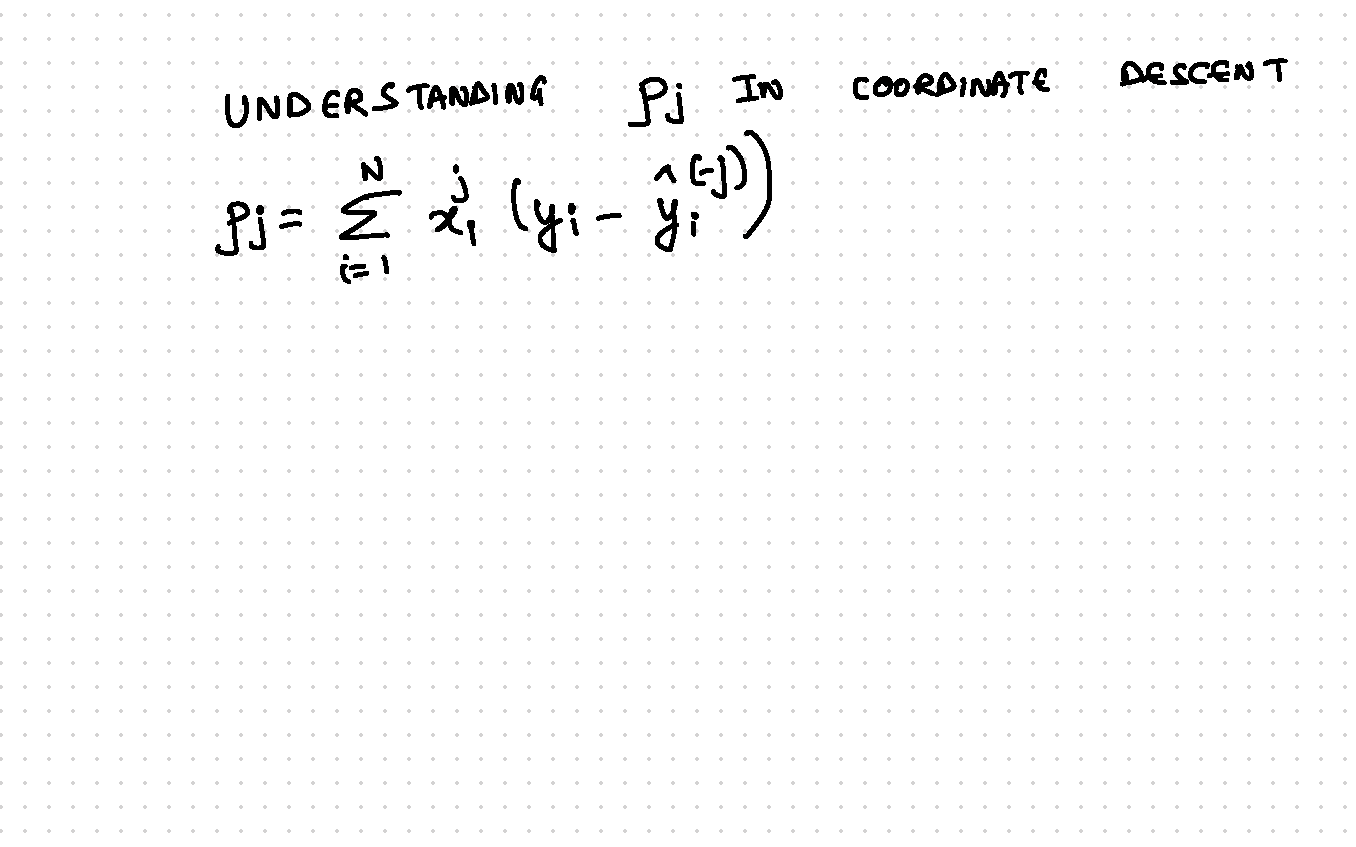
\includepdf[page=-]{coordinate-rho.pdf}
}




\begin{frame}{Coordinate Descent for Lasso Regression}
\[
  \text{Minimize} \underbrace{\sum_{i=1}^{N} \epsilon^{2} + \delta^{2}\left\{\left|\theta_{0}\right|+\left|\theta_{1}\right|+\ldots\left|\theta_{j}\right|+\ldots |\theta_{d}|\right\}}_{LASSO \: OBJECTIVE}
\]
\begin{align*}
\frac{\partial}{\partial \theta_{j}}(& \text {LASSO OBJECTIVE})=-2 \rho_{j}+2 \theta_{j} z_{j}+\delta^{2}{\frac{\partial}{\partial \theta_{j}}}\left|\theta_{j}\right|\\[18pt]
&\frac{\partial}{\partial \theta_{j}}\left|\theta_{j}\right|=\left\{\begin{array}{cc}
{1} & {\theta_{j}>0} \\
{[-1,1]} & {\theta_{j}=0} \\
{-1} & {\theta_{j}<0}
\end{array}\right.
\end{align*}
\end{frame}

\begin{frame}{Coordinate Descent for Lasso Regression}
\begin{itemize}[<+->]
    \item \textbf{Case 1: $\theta_{j}>0$}
    \begin{align*}
    \-2\rho_j+2\theta_j z_j+\delta^{2}  = 0\\
    \theta_j = \frac{\rho_j - \frac{\delta^{2}}{2}}{z_{j}}\\
    \rho_{j}>\frac{\delta^{2}}{2} \Rightarrow  \theta_{j} = \frac{\rho_j - \frac{\delta^{2}}{2}}{z_{j}}
    \end{align*}
    
   \item \textbf{Case 2: $\theta_{j}<0$}
    \begin{equation}
        \rho_{j} < \frac{\delta^{2}}{2} \Rightarrow \theta_{j} = \frac{\rho_{j}+\delta^{2} / 2}{z_{j}}
    \end{equation}
\end{itemize}
    
\end{frame}

\begin{frame}{Coordinate Descent for Lasso Regression}
\begin{itemize}
    \item \textbf{Case 3: $\theta_{j} = 0$}
    \begin{align*}
    \frac{\partial}{\partial \theta_{j}}(\text {LASSO OBJECTIVE})&=-2 \rho_{j}+2\theta_{j} z_{j}+ \delta^{2}\underbrace{{\frac{\partial}{\partial \theta_{j}}}\left|\theta_{j}\right|}_{\text{[-1,1]}}\\
    &\epsilon \underbrace{[-2\rho_{j} - \delta^{2}, -2\rho_{j} + \delta^{2}]}_{\text{$\{0\}$ lies in this range}}\\
    \end{align*}
    \begin{align*}
    -2\rho_{j} - \delta^{2} \leq 0 \text{ and }& -2\rho_{j} - \delta^{2} \leq 0\\
    -\frac{\delta^{2}}{2} \leq \rho_j \leq \frac{\delta^{2}}{2}  \Rightarrow & \hspace{2mm} \theta_{j}=0
    \end{align*}
    
\end{itemize}
    
\end{frame}
\begin{frame}{Summary of Lasso Regression}
\begin{equation}
\theta_{j} =\left[\begin{array}{ccc}
{\frac{\rho_{j} + \frac{\delta^{2}}{2}}{z_{j}}} & {if}  & {\rho_{j}<-\frac{\delta^{2}}{2}} \\
{0} & {if} & {-\frac{\delta^{2}}{2} \leq \rho_{j} \leq \frac{\delta^{2}}{2}} \\
{\frac{\rho_{j} - \frac{\delta^{2}}{2}}{z_{j}}} & {i f} & {\rho_{j}>\frac{\delta^{2}}{2}}
\end{array}\right]
\end{equation}
    
\end{frame}

{
	\setbeamercolor{background canvas}{bg=}
	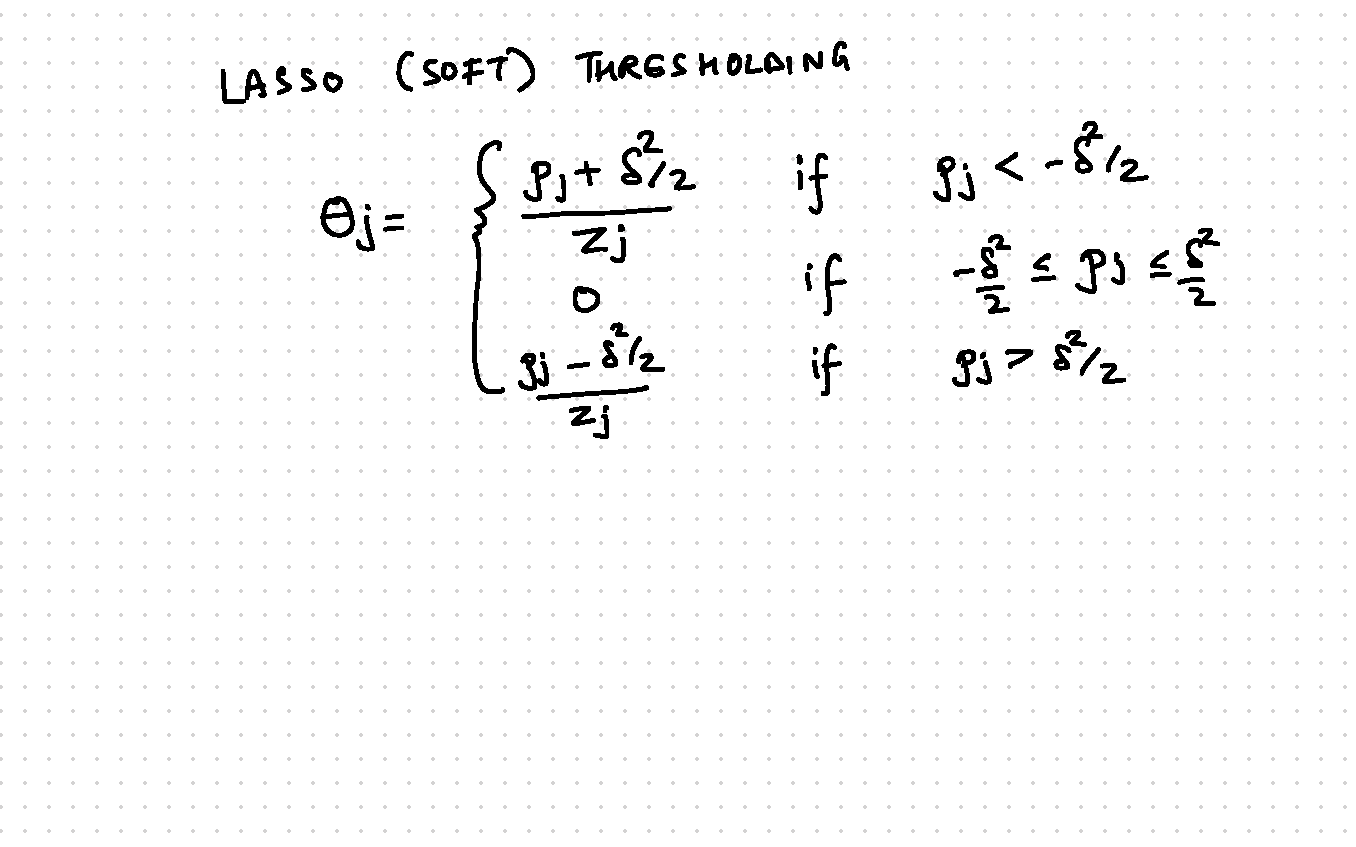
\includepdf[page=-]{coordinate-thresholding.pdf}
}
\end{document}